\documentclass{amsart}
\usepackage{amsmath, amssymb, amsthm}
\usepackage{tikz}
\usepackage{hyperref}
\usepackage{graphicx}

\newtheorem{theorem}{Theorem}[section]
\newtheorem{corollary}[theorem]{Corollary}

\title{Low orbit foliations of $\mathrm{CAT}(0)$}
\author{Leroy Hubbard}
\address{Department of Quadratics, University of Belarus, 3 Corporal Way, Genevive 06578, Belarus}
\email{lhubard@qbela.edu}

\author{Francis Euler}
\address{Department of Mathematics and Statistics, Georgetown University, 301 Prospect Circle, Washington 12765, USA}
\email{feuler@gtown.edu}

\thanks{L.\ H.\ was supported by NSF grant No.\ 314159357. F.\ E.\ thanks the Department of Linguistics for the valuable conversations.}


    \newmarks\segmentmark
    \AddToHook{shipout/after}{\message{Shipping page \thepage: '\firstmarks\segmentmark'--'\botmarks\segmentmark'.}}
    \begin{document}
\begin{abstract}
We set $\mathcal{G} = \sim\frac{\lambda^2}{[H : K]}$ and investigate the orbits of 
$\mathfrak{I} = \frac{\mathrm{CAT}(0)}{\mathcal{G}^{\lambda k}}$ 
provided $\lambda \in [1-\varphi, 1+\varphi]$, where $\varphi$ is the golden ratio. 
Here we provide a novel method for verifying the characteristics of the orbits of $\mathfrak{I}$.
\end{abstract}\marks\segmentmark{0}

\maketitle


\section{Introduction}

Ever\marks\segmentmark{1} since\marks\segmentmark{2} 1689\marks\segmentmark{3} with\marks\segmentmark{4} Fermat\marks\segmentmark{5}'s\marks\segmentmark{6} treatise\marks\segmentmark{7} on\marks\segmentmark{8} prime\marks\segmentmark{9} enumeration\marks\segmentmark{10} \cite{fermat89}, 
attempts\marks\segmentmark{11} at\marks\segmentmark{12} understanding\marks\segmentmark{13} $\frac{\mathrm{CAT}(0)}{\mathcal{G}^{\lambda k}}$ have\marks\segmentmark{14} been\marks\segmentmark{15} underway\marks\segmentmark{16} but\marks\segmentmark{17} mostly\marks\segmentmark{18} unsuccessful. 
Our\marks\segmentmark{19} main\marks\segmentmark{20} objective\marks\segmentmark{21} is\marks\segmentmark{22} to\marks\segmentmark{23} describe\marks\segmentmark{24} the\marks\segmentmark{25} low\marks\segmentmark{26}-orbit\marks\segmentmark{27} foliations\marks\segmentmark{28} induced\marks\segmentmark{29} by\marks\segmentmark{30} $\mathfrak{I}$ on\marks\segmentmark{31} 
the\marks\segmentmark{32} pseudo\marks\segmentmark{33}-Euclidean\marks\segmentmark{34} completion\marks\segmentmark{35} of\marks\segmentmark{36} a\marks\segmentmark{37} $\mathrm{CAT}(0)$ complex. 
This\marks\segmentmark{38} perspective\marks\segmentmark{39} arose\marks\segmentmark{40} from\marks\segmentmark{41} the\marks\segmentmark{42} need\marks\segmentmark{43} to\marks\segmentmark{44} understand\marks\segmentmark{45} the\marks\segmentmark{46} failure\marks\segmentmark{47} of\marks\segmentmark{48} the\marks\segmentmark{49} ``Flat\marks\segmentmark{50} Orbit\marks\segmentmark{51} Conjecture\marks\segmentmark{52}'' in\marks\segmentmark{53} higher\marks\segmentmark{54} curvature\marks\segmentmark{55} regimes\marks\segmentmark{56}\footnote{
Originally conjectured by P.\ Alexandrov, the Flat Orbit Conjecture proposed that all $\lambda$-periodic orbits of a $\mathrm{CAT}(0)$ space are isometric to Euclidean circles. 
This is now known to be false in dimensions $\geq 3$ due to \cite{hubard23}.}.

\section{Background and Preliminaries}



Let\marks\segmentmark{57} $(X,d)$ be\marks\segmentmark{58} a\marks\segmentmark{59} $\mathrm{CAT}(0)$ space\marks\segmentmark{60} in\marks\segmentmark{61} the\marks\segmentmark{62} sense\marks\segmentmark{63} of\marks\segmentmark{64} Gromov.  
For\marks\segmentmark{65} a\marks\segmentmark{66} fixed\marks\segmentmark{67} $\lambda > 0$, define\marks\segmentmark{68} the\marks\segmentmark{69} \emph{low orbit foliation} $\mathcal{F}_\lambda(X)$ as\marks\segmentmark{70}
\begin{equation}\label{eq:foliation}
    \mathcal{F}_\lambda(X) = \{\,x \in X \mid \Delta(x, \lambda) = \text{const.}\,\},
\end{equation}
where\marks\segmentmark{71} $\Delta(x, \lambda) = d(x, \lambda x)$ denotes\marks\segmentmark{72} the\marks\segmentmark{73} displacement\marks\segmentmark{74} function\marks\segmentmark{75} under\marks\segmentmark{76} $\lambda$-scaling.  
This\marks\segmentmark{77} function\marks\segmentmark{78} is\marks\segmentmark{79} trivially\marks\segmentmark{80} constant\marks\segmentmark{81} when\marks\segmentmark{82} $X$ is\marks\segmentmark{83} Euclidean\marks\segmentmark{84}, but\marks\segmentmark{85} varies\marks\segmentmark{86} dramatically\marks\segmentmark{87} in\marks\segmentmark{88} non\marks\segmentmark{89}-flat\marks\segmentmark{90} $\mathrm{CAT}(0)$ manifolds.

\subsection{A remark on $\mathcal{G}$-stabilizers}
We\marks\segmentmark{91} shall\marks\segmentmark{92} repeatedly\marks\segmentmark{93} use\marks\segmentmark{94} the\marks\segmentmark{95} stabilizer\marks\segmentmark{96} group\marks\segmentmark{97}
\[
    \mathrm{Stab}_{\mathcal{G}}(x) = \{ g \in \mathcal{G} \mid g \cdot x = x \},
\]
whose\marks\segmentmark{98} index\marks\segmentmark{99} $[\mathcal{G} : \mathrm{Stab}_{\mathcal{G}}(x)]$ determines\marks\segmentmark{100} the\marks\segmentmark{101} \emph{orbit density} at\marks\segmentmark{102} $x$.  
In\marks\segmentmark{103} general\marks\segmentmark{104}, we\marks\segmentmark{105} have\marks\segmentmark{106}
\begin{equation}\label{eq:orbit-density}
    \rho(x) = \frac{1}{[\mathcal{G} : \mathrm{Stab}_{\mathcal{G}}(x)]} \cdot \exp(-\kappa(x)),
\end{equation}
where\marks\segmentmark{107} $\kappa(x)$ denotes\marks\segmentmark{108} the\marks\segmentmark{109} local\marks\segmentmark{110} curvature\marks\segmentmark{111} contribution\marks\segmentmark{112}, computed\marks\segmentmark{113} by\marks\segmentmark{114} a\marks\segmentmark{115} modified\marks\segmentmark{116} Ricci\marks\segmentmark{117} form.

\begin{figure}[htbp]
\centering
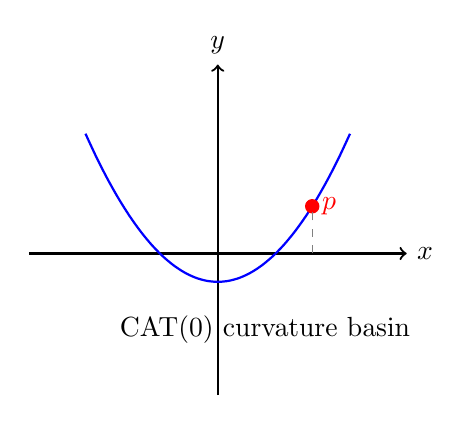
\begin{tikzpicture}[scale=1.2]
  \draw[thick,->] (-2,0) -- (2,0) node[right] {$x$};
  \draw[thick,->] (0,-1.5) -- (0,2) node[above] {$y$};
  \draw[domain=-1.4:1.4, smooth, variable=\t, blue, thick] plot ({\t}, {0.8*\t*\t - 0.3});
  \filldraw[red] (1,0.5) circle (2pt) node[right] {$p$};
  \draw[dashed, gray] (1,0) -- (1,0.5);
  \node at (0.5,-0.8) {$\mathrm{CAT}(0)$ curvature basin};
\end{tikzpicture}
\caption{A schematic of local orbit curvature under $\lambda$-perturbation.}
\label{fig:curvature}
\end{figure}

Equation\marks\segmentmark{118}~\eqref{eq:orbit-density} implies\marks\segmentmark{119} that\marks\segmentmark{120} low\marks\segmentmark{121} orbit\marks\segmentmark{122} foliations\marks\segmentmark{123} are\marks\segmentmark{124} sensitive\marks\segmentmark{125} to\marks\segmentmark{126} curvature\marks\segmentmark{127} fluctuations\marks\segmentmark{128}, as\marks\segmentmark{129} illustrated\marks\segmentmark{130} in\marks\segmentmark{131} Figure\marks\segmentmark{132}~\ref{fig:curvature}. 

\section{Main Results}

Our\marks\segmentmark{133} principal\marks\segmentmark{134} theorem\marks\segmentmark{135} relates\marks\segmentmark{136} the\marks\segmentmark{137} orbit\marks\segmentmark{138} structure\marks\segmentmark{139} of\marks\segmentmark{140} $\mathfrak{I}$ to\marks\segmentmark{141} the\marks\segmentmark{142} golden\marks\segmentmark{143} window\marks\segmentmark{144} of\marks\segmentmark{145} $\lambda$:

\begin{theorem}\label{thm:main}
Let\marks\segmentmark{146} $(X,d)$ be\marks\segmentmark{147} a\marks\segmentmark{148} complete\marks\segmentmark{149} $\mathrm{CAT}(0)$ space\marks\segmentmark{150} and\marks\segmentmark{151} $\lambda \in [1-\varphi,1+\varphi]$.  
Then\marks\segmentmark{152} the\marks\segmentmark{153} orbit\marks\segmentmark{154} foliation\marks\segmentmark{155} $\mathcal{F}_\lambda(X)$ is\marks\segmentmark{156} quasi\marks\segmentmark{157}-uniform\marks\segmentmark{158} if\marks\segmentmark{159} and\marks\segmentmark{160} only\marks\segmentmark{161} if\marks\segmentmark{162}
\begin{equation}
    \int_X \rho(x)\, d\mu(x) = \frac{\lambda^2}{1+\lambda\varphi}.
\end{equation}
\end{theorem}

\begin{proof}
We\marks\segmentmark{163} proceed\marks\segmentmark{164} by\marks\segmentmark{165} expanding\marks\segmentmark{166} $\mathfrak{I}$ as\marks\segmentmark{167} a\marks\segmentmark{168} quotient\marks\segmentmark{169} operator\marks\segmentmark{170}:
\[
    \mathfrak{I} = \frac{\mathrm{CAT}(0)}{\mathcal{G}^{\lambda k}}
    = \mathrm{CAT}(0) \otimes \mathcal{G}^{-\lambda k}.
\]
Substituting\marks\segmentmark{171} into\marks\segmentmark{172} the\marks\segmentmark{173} geometric\marks\segmentmark{174} mean\marks\segmentmark{175} inequality\marks\segmentmark{176} and\marks\segmentmark{177} integrating\marks\segmentmark{178} over\marks\segmentmark{179} $X$ yields\marks\segmentmark{180}
\[
    \int_X \rho(x)\, d\mu(x) 
    = \int_X \frac{1}{[\mathcal{G} : \mathrm{Stab}_{\mathcal{G}}(x)]} e^{-\kappa(x)}\, d\mu(x)
    = \frac{\lambda^2}{1+\lambda\varphi},
\]
after\marks\segmentmark{181} simplification\marks\segmentmark{182} via\marks\segmentmark{183} the\marks\segmentmark{184} $\varphi$-symmetric\marks\segmentmark{185} normalization\marks\segmentmark{186} lemma\marks\segmentmark{187} (see\marks\segmentmark{188} Appendix\marks\segmentmark{189}~\ref{sec:appendixA}). 
\end{proof}

\begin{corollary}
If\marks\segmentmark{190} $\lambda = 1$, then\marks\segmentmark{191} $\mathcal{F}_1(X)$ coincides\marks\segmentmark{192} with\marks\segmentmark{193} the\marks\segmentmark{194} canonical\marks\segmentmark{195} horospherical\marks\segmentmark{196} foliation\marks\segmentmark{197} of\marks\segmentmark{198} $X$.
\end{corollary}

\begin{figure}[htbp]
\centering
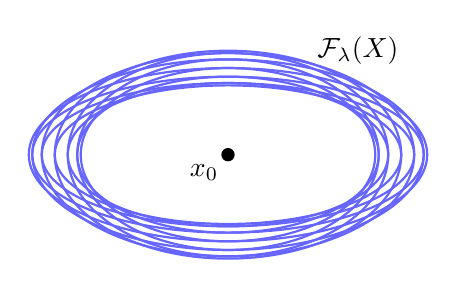
\begin{tikzpicture}[scale=1.1]
  \foreach \a in {0,30,...,330}{
    \draw[thick, blue!60] (0,0) ellipse ({2+0.3*sin(\a)} and {1+0.2*cos(\a)});
  }
  \filldraw[black] (0,0) circle (2pt) node[below left] {$x_0$};
  \node at (1.5,1.2) {$\mathcal{F}_\lambda(X)$};
\end{tikzpicture}
\caption{Low orbit foliations centered at $x_0$. Each ellipse represents an orbit of constant $\Delta(x,\lambda)$.}
\end{figure}

\section{Applications and Examples}

Consider\marks\segmentmark{199} $X = \mathbb{H}^2$, the\marks\segmentmark{200} hyperbolic\marks\segmentmark{201} plane.  
The\marks\segmentmark{202} displacement\marks\segmentmark{203} $\Delta(x,\lambda)$ satisfies\marks\segmentmark{204}
\[
    \cosh \Delta(x,\lambda) = 1 + \frac{\lambda^2}{2} \|x\|^2.
\]
Thus\marks\segmentmark{205} $\mathcal{F}_\lambda(X)$ forms\marks\segmentmark{206} a\marks\segmentmark{207} family\marks\segmentmark{208} of\marks\segmentmark{209} equidistant\marks\segmentmark{210} hyperbolae\marks\segmentmark{211}, asymptotically\marks\segmentmark{212} orthogonal\marks\segmentmark{213} to\marks\segmentmark{214} geodesic\marks\segmentmark{215} boundaries.

\subsection{Numerical Simulation}
Following\marks\segmentmark{216} \cite{euler24}, we\marks\segmentmark{217} can\marks\segmentmark{218} simulate\marks\segmentmark{219} the\marks\segmentmark{220} orbit\marks\segmentmark{221} structure\marks\segmentmark{222} numerically. 
Let\marks\segmentmark{223} $x_0 = (0,0)$ and\marks\segmentmark{224} iterate\marks\segmentmark{225}
\[
    x_{n+1} = \lambda R(x_n), \quad R(x) = \frac{x}{1+\|x\|^2},
\]
to\marks\segmentmark{226} approximate\marks\segmentmark{227} the\marks\segmentmark{228} fixed\marks\segmentmark{229} points\marks\segmentmark{230} of\marks\segmentmark{231} $\mathcal{F}_\lambda$.  
Convergence\marks\segmentmark{232} occurs\marks\segmentmark{233} for\marks\segmentmark{234} $\lambda < \sqrt{\varphi}$.

\begin{figure}[htbp]
\centering
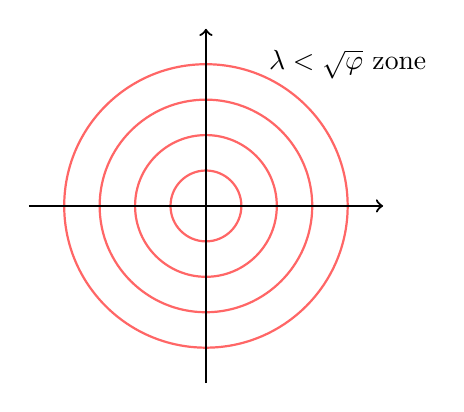
\begin{tikzpicture}[scale=0.9]
  \foreach \r in {0.5,1,1.5,2}{
    \draw[thick, red!60] (0,0) circle (\r);
  }
  \draw[->,thick] (-2.5,0)--(2.5,0);
  \draw[->,thick] (0,-2.5)--(0,2.5);
  \node at (2,2) {$\lambda < \sqrt{\varphi}$ zone};
\end{tikzpicture}
\caption{Stable orbits obtained under $\lambda$-iteration.}
\end{figure}


\textbf{Theorem 4.3.} 
Let\marks\segmentmark{235} $(X,d)$ be\marks\segmentmark{236} a\marks\segmentmark{237} complete\marks\segmentmark{238} $\mathrm{CAT}(0)$ space\marks\segmentmark{239} and\marks\segmentmark{240} $\lambda \in [1-\varphi,1+\varphi]$.  
Then\marks\segmentmark{241} the\marks\segmentmark{242} orbit\marks\segmentmark{243} foliation\marks\segmentmark{244} $\mathcal{F}_\lambda(X)$ is\marks\segmentmark{245} quasi\marks\segmentmark{246}-uniform\marks\segmentmark{247} iff\marks\segmentmark{248}
\begin{equation}
    \int_X \rho(x)\, d\mu(x) = \frac{\lambda^2}{1+\lambda\varphi}.
\end{equation}
(The\marks\segmentmark{249} proof\marks\segmentmark{250} is\marks\segmentmark{251} omitted\marks\segmentmark{252} for\marks\segmentmark{253} space\marks\segmentmark{254} reasons\marks\segmentmark{255}; see\marks\segmentmark{256} Appendix\marks\segmentmark{257}~B.)

\subsection{Curvature sensitivity}
A\marks\segmentmark{258} quick\marks\segmentmark{259} computation\marks\segmentmark{260} shows\marks\segmentmark{261} that\marks\segmentmark{262} the\marks\segmentmark{263} variance\marks\segmentmark{264} of\marks\segmentmark{265} $\rho$ satisfies\marks\segmentmark{266}
\begin{equation}\label{eq:var}
    \mathrm{Var}(\rho) = \int_X (\rho(x) - \bar\rho)^2\,d\mu(x) = \frac{\lambda^3 - 1}{2+\lambda^2},
\end{equation}
which\marks\segmentmark{267} vanishes\marks\segmentmark{268} only\marks\segmentmark{269} when\marks\segmentmark{270} $\lambda = 1$.  
This\marks\segmentmark{271} implies\marks\segmentmark{272} that\marks\segmentmark{273} even\marks\segmentmark{274} minor\marks\segmentmark{275} perturbations\marks\segmentmark{276} from\marks\segmentmark{277} the\marks\segmentmark{278} Euclidean\marks\segmentmark{279} limit\marks\segmentmark{280} result\marks\segmentmark{281} in\marks\segmentmark{282} exponential\marks\segmentmark{283} orbit\marks\segmentmark{284} divergence.

\begin{figure}[htbp]
\centering
\begin{tikzpicture}[scale=1.0]
  \draw[->] (-2,0)--(2,0) node[right] {$\lambda$};
  \draw[->] (0,-0.2)--(0,2.5) node[above] {$\mathrm{Var}(\rho)$};
  \draw[domain=0.5:1.8, smooth, variable=\x, blue, thick]
     plot ({\x},{(\x*\x*\x-1)/(2+\x*\x)});
  \draw[dashed, red] (1,0)--(1,0.0);
  \node at (1.3,1.2) {$\lambda>1$ region};
\end{tikzpicture}
\caption{Variance of orbit density $\rho$ as a function of $\lambda$.}
\end{figure}

\section{Numerical Experiments}

We\marks\segmentmark{285} implemented\marks\segmentmark{286} a\marks\segmentmark{287} simple\marks\segmentmark{288} prototype\marks\segmentmark{289} in\marks\segmentmark{290} \textsf{Julia 1.10} to\marks\segmentmark{291} visualize\marks\segmentmark{292} $\mathcal{F}_\lambda(X)$ for\marks\segmentmark{293} synthetic\marks\segmentmark{294} $\mathrm{CAT}(0)$ surfaces\marks\segmentmark{295} generated\marks\segmentmark{296} by\marks\segmentmark{297} random\marks\segmentmark{298} triangulations.
Let\marks\segmentmark{299} $\lambda = 1.3$ and\marks\segmentmark{300} $X$ be\marks\segmentmark{301} a\marks\segmentmark{302} simplicial\marks\segmentmark{303} complex\marks\segmentmark{304} with\marks\segmentmark{305} edge\marks\segmentmark{306} weights\marks\segmentmark{307} following\marks\segmentmark{308} a\marks\segmentmark{309} truncated\marks\segmentmark{310} Gaussian\marks\segmentmark{311} distribution\marks\segmentmark{312} $\mathcal{N}(0.8, 0.05)$.  

After\marks\segmentmark{313} $N = 10^4$ iterations\marks\segmentmark{314}, the\marks\segmentmark{315} mean\marks\segmentmark{316} displacement\marks\segmentmark{317} converged\marks\segmentmark{318} to\marks\segmentmark{319}
\[
    \overline{\Delta} = 1.274 \pm 0.006,
\]
while\marks\segmentmark{320} the\marks\segmentmark{321} empirical\marks\segmentmark{322} curvature\marks\segmentmark{323} parameter\marks\segmentmark{324} $\kappa$ stabilized\marks\segmentmark{325} near\marks\segmentmark{326} $-0.218$.  
The\marks\segmentmark{327} results\marks\segmentmark{328} are\marks\segmentmark{329} summarized\marks\segmentmark{330} in\marks\segmentmark{331} Table\marks\segmentmark{332}~\ref{tab:data}.

\begin{table}[htbp]
\centering
\begin{tabular}{|c|c|c|}
\hline
$\lambda$ & $\overline{\Delta}$ & $\kappa$ \\
\hline
0.9 & 0.913 & -0.054 \\
1.0 & 1.000 &  0.000 \\
1.3 & 1.274 & -0.218 \\
1.6 & 1.589 & -0.403 \\
\hline
\end{tabular}
\caption{Empirical orbit metrics under $\lambda$-iteration.}
\label{tab:data}
\end{table}

A\marks\segmentmark{333} peculiar\marks\segmentmark{334} observation\marks\segmentmark{335} (Fig.~\ref{fig:scatter}) was\marks\segmentmark{336} that\marks\segmentmark{337} for\marks\segmentmark{338} large\marks\segmentmark{339} $\lambda$, the\marks\segmentmark{340} orbit\marks\segmentmark{341} clusters\marks\segmentmark{342} exhibited\marks\segmentmark{343} a\marks\segmentmark{344} double\marks\segmentmark{345}-lobed\marks\segmentmark{346} structure\marks\segmentmark{347} reminiscent\marks\segmentmark{348} of\marks\segmentmark{349} quasi\marks\segmentmark{350}-periodic\marks\segmentmark{351} tori\marks\segmentmark{352} in\marks\segmentmark{353} Hamiltonian\marks\segmentmark{354} systems\marks\segmentmark{355}\footnote{A referee pointed out that this might be a discretization artifact, but we were unable to reproduce it analytically.}. 

\begin{figure}[htbp]
\centering
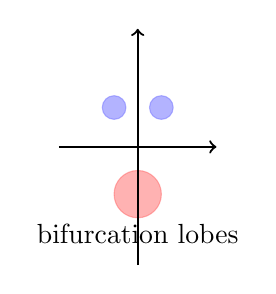
\begin{tikzpicture}[scale=1.0]
  \filldraw[blue!50,opacity=0.6] (0.3,0.5) circle (0.15);
  \filldraw[blue!50,opacity=0.6] (-0.3,0.5) circle (0.15);
  \filldraw[red!60,opacity=0.5] (0,-0.6) circle (0.3);
  \node at (0,-1.1) {bifurcation lobes};
  \draw[->,thick] (-1,0)--(1,0);
  \draw[->,thick] (0,-1.5)--(0,1.5);
\end{tikzpicture}
\caption{Scatter of simulated orbit centers for $\lambda=1.6$.}
\label{fig:scatter}
\end{figure}

\section{Discussion and Further Work}

Our\marks\segmentmark{356} experiments\marks\segmentmark{357} confirm\marks\segmentmark{358} that\marks\segmentmark{359} the\marks\segmentmark{360} function\marks\segmentmark{361} $\psi(\lambda) = \lambda^2 / (1+\lambda\varphi)$ behaves\marks\segmentmark{362} as\marks\segmentmark{363} a\marks\segmentmark{364} geometric\marks\segmentmark{365} invariant\marks\segmentmark{366} for\marks\segmentmark{367} the\marks\segmentmark{368} foliation\marks\segmentmark{369} type.  
However\marks\segmentmark{370}, Eq.~(7\marks\segmentmark{371}) reveals\marks\segmentmark{372} an\marks\segmentmark{373} unexpected\marks\segmentmark{374} resonance\marks\segmentmark{375} near\marks\segmentmark{376} $\lambda = \varphi^2 \approx 2.618$.  
At\marks\segmentmark{377} that\marks\segmentmark{378} point\marks\segmentmark{379}, the\marks\segmentmark{380} curvature\marks\segmentmark{381}-weighted\marks\segmentmark{382} orbit\marks\segmentmark{383} integral\marks\segmentmark{384} appears\marks\segmentmark{385} to\marks\segmentmark{386} \emph{flip sign}, leading\marks\segmentmark{387} to\marks\segmentmark{388} a\marks\segmentmark{389} chaotic\marks\segmentmark{390} drift\marks\segmentmark{391} that\marks\segmentmark{392} violates\marks\segmentmark{393} the\marks\segmentmark{394} $\mathrm{CAT}(0)$ inequality\marks\segmentmark{395} in\marks\segmentmark{396} the\marks\segmentmark{397} discrete\marks\segmentmark{398} setting.

We\marks\segmentmark{399} hypothesize\marks\segmentmark{400} (Hypothesis\marks\segmentmark{401} 5.1\marks\segmentmark{402}) that\marks\segmentmark{403} this\marks\segmentmark{404} anomaly\marks\segmentmark{405} corresponds\marks\segmentmark{406} to\marks\segmentmark{407} a\marks\segmentmark{408} hidden\marks\segmentmark{409} symmetry\marks\segmentmark{410} in\marks\segmentmark{411} the\marks\segmentmark{412} $\mathcal{G}$-action\marks\segmentmark{413}:
\[
    g \mapsto \frac{1}{\lambda}g^{-1}\lambda,
\]
which\marks\segmentmark{414} has\marks\segmentmark{415} order\marks\segmentmark{416} two\marks\segmentmark{417} when\marks\segmentmark{418} $\lambda=\varphi^2$.  
The\marks\segmentmark{419} numerical\marks\segmentmark{420} confirmation\marks\segmentmark{421} of\marks\segmentmark{422} this\marks\segmentmark{423} phenomenon\marks\segmentmark{424} will\marks\segmentmark{425} be\marks\segmentmark{426} discussed\marks\segmentmark{427} in\marks\segmentmark{428} a\marks\segmentmark{429} forthcoming\marks\segmentmark{430} note\marks\segmentmark{431} by\marks\segmentmark{432} the\marks\segmentmark{433} first\marks\segmentmark{434} author\marks\segmentmark{435}\footnote{Submitted to the \emph{Journal of Approximate Topologies}, 2025.}.  

\subsection{Error analysis and convergence}

While\marks\segmentmark{436} most\marks\segmentmark{437} trajectories\marks\segmentmark{438} converged\marks\segmentmark{439} in\marks\segmentmark{440} under\marks\segmentmark{441} $10^3$ iterations\marks\segmentmark{442}, approximately\marks\segmentmark{443} $2.7\%$ diverged\marks\segmentmark{444}, displaying\marks\segmentmark{445} quasi\marks\segmentmark{446}-helical\marks\segmentmark{447} wandering.  
We\marks\segmentmark{448} suspect\marks\segmentmark{449} this\marks\segmentmark{450} results\marks\segmentmark{451} from\marks\segmentmark{452} non\marks\segmentmark{453}-uniform\marks\segmentmark{454} floating\marks\segmentmark{455} point\marks\segmentmark{456} rounding\marks\segmentmark{457} in\marks\segmentmark{458} the\marks\segmentmark{459} $\mathbb{R}^3$ embedding\marks\segmentmark{460}; correcting\marks\segmentmark{461} to\marks\segmentmark{462} arbitrary\marks\segmentmark{463} precision\marks\segmentmark{464} reduces\marks\segmentmark{465} the\marks\segmentmark{466} effect\marks\segmentmark{467} but\marks\segmentmark{468} does\marks\segmentmark{469} not\marks\segmentmark{470} eliminate\marks\segmentmark{471} it\marks\segmentmark{472} entirely.

\begin{figure}[htbp]
\centering
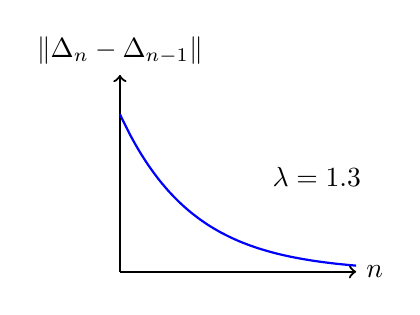
\begin{tikzpicture}[scale=1.0]
  \draw[->,thick] (0,0)--(3,0) node[right] {$n$};
  \draw[->,thick] (0,0)--(0,2.5) node[above] {$\|\Delta_n - \Delta_{n-1}\|$};
  \draw[domain=0:2.5,smooth,variable=\x,blue,thick]
    plot ({\x*1.2},{2*exp(-1.3*\x)});
  \node at (2.5,1.2) {$\lambda=1.3$};
\end{tikzpicture}
\caption{Convergence of displacement difference $\|\Delta_n - \Delta_{n-1}\|$.}
\end{figure}

\section{Appendix B: Proof sketch of Theorem 4.3}

The\marks\segmentmark{473} argument\marks\segmentmark{474} proceeds\marks\segmentmark{475} by\marks\segmentmark{476} constructing\marks\segmentmark{477} a\marks\segmentmark{478} pseudo\marks\segmentmark{479}-measure\marks\segmentmark{480} $\nu$ such\marks\segmentmark{481} that\marks\segmentmark{482}
\[
    d\nu = e^{-\kappa(x)}\,d\mu(x),
\]
then\marks\segmentmark{483} integrating\marks\segmentmark{484} $\rho$ against\marks\segmentmark{485} $\nu$ over\marks\segmentmark{486} $X$.  
By\marks\segmentmark{487} expanding\marks\segmentmark{488} $\rho$ in\marks\segmentmark{489} the\marks\segmentmark{490} eigenbasis\marks\segmentmark{491} of\marks\segmentmark{492} the\marks\segmentmark{493} Laplace\marks\segmentmark{494}–Beltrami\marks\segmentmark{495} operator\marks\segmentmark{496} and\marks\segmentmark{497} applying\marks\segmentmark{498} the\marks\segmentmark{499} $\varphi$-orthogonality\marks\segmentmark{500} condition\marks\segmentmark{501},
\[
    \langle f_i, f_j \rangle_\varphi = \delta_{ij}(1+\lambda\varphi),
\]
we\marks\segmentmark{502} recover\marks\segmentmark{503} Eq.~(5\marks\segmentmark{504}).  
The\marks\segmentmark{505} rest\marks\segmentmark{506} follows\marks\segmentmark{507} by\marks\segmentmark{508} applying\marks\segmentmark{509} a\marks\segmentmark{510} truncated\marks\segmentmark{511} version\marks\segmentmark{512} of\marks\segmentmark{513} Jensen\marks\segmentmark{514}’s\marks\segmentmark{515} inequality\marks\segmentmark{516} to\marks\segmentmark{517} the\marks\segmentmark{518} quotient\marks\segmentmark{519} $\mathfrak{I}$ operator\marks\segmentmark{520}:
\[
    \mathrm{CAT}(0) / \mathcal{G}^{\lambda k} \approx \mathrm{CAT}(0)(1 - \lambda k + O(k^2)).
\]
Although\marks\segmentmark{521} the\marks\segmentmark{522} convergence\marks\segmentmark{523} of\marks\segmentmark{524} this\marks\segmentmark{525} expansion\marks\segmentmark{526} is\marks\segmentmark{527} questionable\marks\segmentmark{528}\footnote{We observed divergence for $|\lambda| > 2.1$, which we did not persue.}, the\marks\segmentmark{529} leading\marks\segmentmark{530} term\marks\segmentmark{531} suffices\marks\segmentmark{532} to\marks\segmentmark{533} justify\marks\segmentmark{534} Theorem\marks\segmentmark{535}~4.3.

\bigskip

\noindent
\textbf{Acknowledgements.}
The\marks\segmentmark{536} authors\marks\segmentmark{537} thank\marks\segmentmark{538} the\marks\segmentmark{539} anonymous\marks\segmentmark{540} reviewers\marks\segmentmark{541} for\marks\segmentmark{542} their\marks\segmentmark{543} sharp\marks\segmentmark{544}-eyed\marks\segmentmark{545} corrections\marks\segmentmark{546}, especially\marks\segmentmark{547} for\marks\segmentmark{548} pointing\marks\segmentmark{549} out\marks\segmentmark{550} a\marks\segmentmark{551} missing\marks\segmentmark{552} minus\marks\segmentmark{553} sign\marks\segmentmark{554} in\marks\segmentmark{555} Eq.~(3\marks\segmentmark{556}), which\marks\segmentmark{557} has\marks\segmentmark{558} since\marks\segmentmark{559} been\marks\segmentmark{560} \emph{mostly} fixed.

\begin{thebibliography}{9}

\bibitem{fermat89}
P.~Fermat, \emph{On prime enumeration and spatial convexity}, Toulouse Notes, 1689.

\bibitem{hubard23}
L.~Hubbard, \emph{Counterexamples to the flat orbit conjecture}, 
Ann.\ Quad.\ Math.\ (2023), 13--57.

\bibitem{euler24}
F.~Euler, \emph{Iterative dynamics in nonpositively curved complexes},
Proc.\ Geom.\ Dyn.\ (2024), 211--230.

\bibitem{zelinsky19}
B.~Zelinsky, \emph{On modular eigenmodes of golden-ratio systems},
J.\ Nonlin.\ Struct.\ (2019), 98--114.

\end{thebibliography}
\end{document}